
\chapter{Results and Discussion}
\label{chap:results-discussion}

\graphicspath{{docs/thesis/figures/chapter4/}{figures/chapter4/}}

\section{Introduction}
\label{sec:results-introduction}

This chapter tests the claims defined in Chapter~\ref{chap:proposed-methodology} using the artifacts produced by the frozen experimental protocol. Evidence is organized around predictive behaviour, serialized encrypted traffic, registered privacy attacks, poisoning response, cryptographic accuracy, and service-level governance. Development choices were fixed before the confirmatory test outputs were interpreted, allowing the reported effects and their limitations to be examined under the same patient partitions and seed pairings.

The confirmatory cohort comprises all 40,336 training-patient files released for the 2019 PhysioNet/Computing in Cardiology Challenge, with the two contributing hospital systems kept separate \cite{reyna2020early,physionet2019sepsis}. Chapter~\ref{chap:proposed-methodology}'s matched-landmark transformation converts each patient's final 24-hour history into 280 input features. The resulting utility matrix contains 125 completed cells. Principal comparisons use ten paired model seeds; computationally heavier SOTA, poisoning, membership-inference, gradient-reconstruction, and ablation analyses use five preselected paired seeds.

Table~\ref{tab:results-environment} summarizes the software and execution environment. The scientific experiments ran on a CPU-based AMD64 Windows 11 workstation. Python, PyTorch, Opacus, NumPy, SciPy, TenSEAL, and Matplotlib were used for training, privacy accounting, numerical analysis, encrypted computation, and visualization. Network-service tests were executed as mutually authenticated processes and Docker containers on one physical host. This distinction is important: the scientific and service profiles validate complementary parts of the framework, but they do not constitute a physical multi-host or wide-area production deployment.

\begin{table}[htbp]
    \centering
    \caption{Experimental software and execution environment}
    \label{tab:results-environment}
    \begin{tabularx}{\textwidth}{@{}lX@{}}
        \toprule
        Item & Recorded configuration \\
        \midrule
        Operating environment & Windows 11, AMD64, CPU-based research workstation \\
        Python and learning stack & CPython 3.13.3; PyTorch 2.13.0+cpu; Opacus 1.6.0 \\
        Numerical and statistical stack & NumPy 2.5.2; SciPy 1.18.1 \\
        Cryptographic stack & TenSEAL 0.3.17 for the main CKKS path; OpenFHE 1.5.1 for the isolated multiparty experiment \\
        Security and visualization & Cryptography 50.0.1; Matplotlib 3.11.1 \\
        Differential-privacy randomness & OS-seeded AES-256-CTR stream, secure Poisson sampling, and four-draw Gaussian construction \\
        Service topology & Hospital, coordinator, authority, and three witness roles on one physical Docker host \\
        Confirmatory cohort & 40,336 patients; two natural hospital partitions; 280 features \\
        \bottomrule
    \end{tabularx}
\end{table}

The chapter is organized in four analytical stages. Section~\ref{sec:quantitative-results} presents predictive, communication, privacy, poisoning, and system measurements. Section~\ref{sec:qualitative-results} reports observed system behaviour under authorization, integrity, failure, and recovery cases. Section~\ref{sec:results-comparative-analysis} compares CAABC-FL with conventional federated methods, encrypted baselines, compression methods, and reproduced SOTA approaches. Finally, Section~\ref{sec:discussion-findings} relates the evidence to the research objectives and states the limitations that bound the conclusions.

\section{Quantitative Results}
\label{sec:quantitative-results}

The quantitative evaluation addresses four questions. First, how much predictive utility is retained after adding patient-level differential privacy, CKKS encryption, and adaptive block compression? Second, does CAABC-FL create a real reduction in serialized encrypted traffic rather than only a reduction in logical coordinates? Third, how does the framework behave under registered privacy and poisoning attacks? Fourth, what computational cost is observed when the protected service is scaled to a larger number of participating clients?

\subsection{Performance Metrics}
\label{subsec:results-metrics}

The classification results were calculated from true positives ($TP$), true negatives ($TN$), false positives ($FP$), and false negatives ($FN$). The resulting accuracy, precision, sensitivity, specificity, and F1 definitions follow standard binary-classification evaluation practice \cite{powers2011evaluation}:

\begin{align}
    \mathrm{Accuracy} &= \frac{TP+TN}{TP+TN+FP+FN}, \label{eq:ch4-accuracy} \\
    \mathrm{Precision} &= \frac{TP}{TP+FP}, \qquad
    \mathrm{Sensitivity} = \frac{TP}{TP+FN}, \label{eq:ch4-precision-recall} \\
    \mathrm{Specificity} &= \frac{TN}{TN+FP}. \label{eq:ch4-specificity}
\end{align}

For this early-sepsis task, sensitivity quantifies how many labelled positive patients are detected, while precision describes how frequently a positive prediction is correct. The F1 statistic combines those two quantities through their harmonic mean,

\begin{equation}
    F1 = 2\frac{\mathrm{Precision}\times\mathrm{Sensitivity}}
    {\mathrm{Precision}+\mathrm{Sensitivity}}.
    \label{eq:ch4-f1}
\end{equation}

AUROC evaluates whether positive examples tend to receive higher scores than negative examples over the range of possible thresholds \cite{fawcett2006roc}. AUPRC instead summarizes the precision--recall relationship and is especially informative for the comparatively rare sepsis outcome \cite{saito2015precision}. Reporting accuracy without these measures could hide a classifier that largely follows the majority class. Every threshold-dependent test metric therefore uses a decision threshold selected once from pooled validation predictions and then held fixed.

Probability quality was assessed with the Brier score \cite{brier1950verification},

\begin{equation}
    \mathrm{Brier}=\frac{1}{N}\sum_{i=1}^{N}(p_i-y_i)^2,
    \label{eq:ch4-brier}
\end{equation}

where $p_i$ is the predicted probability and $y_i\in\{0,1\}$ is the observed label. Lower Brier scores indicate smaller squared probability error. Balanced accuracy and the Matthews correlation coefficient were also computed as secondary measures because they are less dominated by the majority class than ordinary accuracy \cite{powers2011evaluation,chicco2020mcc}.

Communication was measured from serialized ciphertext objects rather than inferred from the number of retained coordinates. Following the communication definition introduced in Equation~\ref{eq:wire-reduction}, if $B_{\mathrm{dense}}$ is the encrypted upload of the dense DP-FedAvg-CKKS reference and $B_m$ is the encrypted upload of method $m$, actual wire reduction is

\begin{equation}
    R_{\mathrm{wire}}(m)=1-\frac{B_m}{B_{\mathrm{dense}}}.
    \label{eq:ch4-wire-reduction}
\end{equation}

This measurement is distinguished from logical payload reduction. A compressor can retain fewer coordinates but still transmit dense ciphertexts, in which case its logical reduction does not become a network saving.

Membership attacks are reported through attack AUROC, following established membership-inference evaluation practice \cite{shokri2017membership,carlini2022membership}. Values close to $0.5$ mean that the registered scoring rule discriminated members from non-members at approximately chance level. Such an empirical result is attack-specific and is not treated as a formal privacy guarantee. Following prior gradient-inversion evaluations \cite{zhu2019dlg,geiping2020inverting}, reconstruction quality is summarized through feature root-mean-square error,

\begin{equation}
    \mathrm{RMSE}=\sqrt{\frac{1}{d}\sum_{j=1}^{d}(\hat{x}_j-x_j)^2},
    \label{eq:ch4-reconstruction-rmse}
\end{equation}

where a larger value indicates poorer reconstruction under the registered optimizer. Poisoning outcomes included change in AUROC, backdoor attack-success-rate (ASR) change, rollback rate, and malicious-client quarantine recall. System performance included serialized upload, encryption time, aggregation time, end-to-end latency, and processed updates per second.

\subsection{Result Tables and Graphical Representations}
\label{subsec:results-tables-figures}

\subsubsection{Predictive performance}

Table~\ref{tab:core-clinical-results} reports the principal clinical metrics. The non-private FedAvg reference achieved an AUROC of $0.830$ and an AUPRC of $0.471$. Introducing patient-level DP produced the expected utility reduction: dense DP-FedAvg-CKKS achieved an AUROC of $0.731$ and an AUPRC of $0.394$. CKKS itself contributed little additional loss relative to plaintext DP-FedAvg, whose corresponding values were $0.732$ and $0.394$. This close agreement is consistent with the small numerical approximation expected from the selected CKKS parameters.

\begin{table}[htbp]
    \centering
    \caption{Core clinical performance on the frozen PhysioNet test partition}
    \label{tab:core-clinical-results}
    \resizebox{\textwidth}{!}{%
    \begin{tabular}{@{}lcccccccc@{}}
        \toprule
        Method & Accuracy & AUROC & AUPRC & Sensitivity & Specificity & Precision & F1 & Brier \\
        \midrule
        FedAvg & 0.729 & 0.830 & 0.471 & 0.757 & 0.726 & 0.182 & 0.292 & 0.157 \\
        DP-FedAvg & 0.832 & 0.732 & 0.394 & 0.458 & 0.861 & 0.224 & 0.293 & 0.064 \\
        DP-FedAvg-CKKS & 0.833 & 0.731 & 0.394 & 0.457 & 0.862 & 0.228 & 0.296 & 0.064 \\
        CAABC-static & 0.815 & 0.732 & 0.390 & 0.476 & 0.841 & 0.210 & 0.282 & 0.065 \\
        CAABC-FL & 0.758 & 0.731 & 0.384 & 0.534 & 0.776 & 0.173 & 0.253 & 0.066 \\
        \bottomrule
    \end{tabular}}
    \vspace{1mm}

    \footnotesize Values are means across ten paired seeds. The privacy-preserving methods used $\epsilon=1.935$ and $\delta=10^{-5}$ under the registered record-level accountant. Threshold-dependent metrics used a validation-selected threshold.
\end{table}

CAABC-FL retained the dense encrypted reference's AUROC but altered its operating-point behaviour. Mean sensitivity increased from $0.457$ to $0.534$, while specificity decreased from $0.862$ to $0.776$. The resulting F1 score declined from $0.296$ to $0.253$. This pattern explains why the apparently higher accuracy of dense DP-FedAvg-CKKS should not be interpreted as uniformly better clinical behaviour: the selected operating point trades fewer false positives for more missed positives. It also shows why both threshold-free and threshold-dependent metrics are necessary.

Figure~\ref{fig:utility-effects} displays paired AUROC and AUPRC effects relative to dense DP-FedAvg-CKKS. The non-private optimizers occupy a different utility region because they do not incur the registered DP mechanism. Among private encrypted methods, most AUROC intervals remain close to zero. CAABC-FL's AUPRC interval lies below zero, making the compression trade-off visible rather than hiding it behind the AUROC result.

\begin{figure}[htbp]
    \centering
    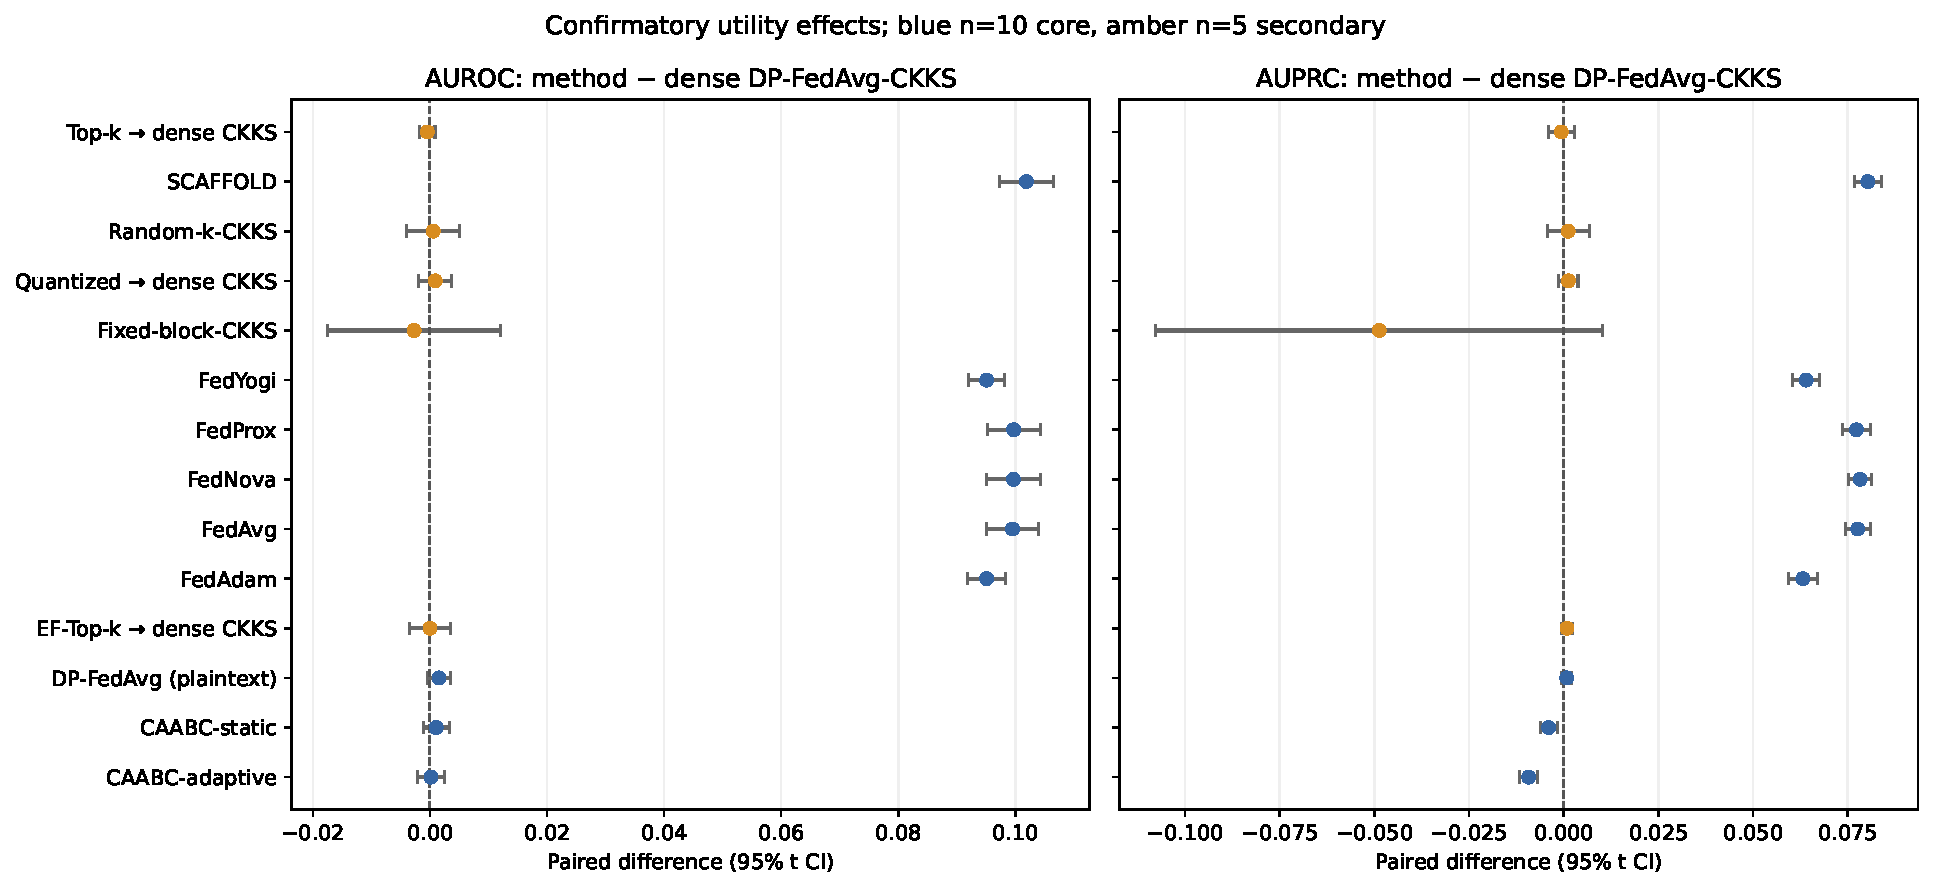
\includegraphics[width=\textwidth]{utility_paired_effect_forest.pdf}
    \caption{Paired differences in AUROC and AUPRC relative to dense DP-FedAvg-CKKS. Blue points use ten core seeds and amber points use five secondary seeds; bars show 95\% confidence intervals.}
    \label{fig:utility-effects}
\end{figure}

\subsubsection{Encrypted communication efficiency}

Table~\ref{tab:communication-results} separates logical compression from actual encrypted-wire reduction. Dense DP-FedAvg-CKKS required approximately $3.314$ MB per round. Top-$k$ and error-feedback Top-$k$ retained fewer logical coordinates but were re-encoded into dense ciphertexts to conceal client-specific supports; consequently, their measured wire reduction was effectively zero. Quantization similarly reduced the logical representation without reducing the serialized CKKS transport.

\begin{table}[htbp]
    \centering
    \caption{Communication cost of privacy-preserving aggregation methods}
    \label{tab:communication-results}
    \resizebox{\textwidth}{!}{%
    \begin{tabular}{@{}lcccc@{}}
        \toprule
        Method & Encrypted upload (MB/round) & Actual wire reduction & Logical reduction & Encrypted transport \\
        \midrule
        DP-FedAvg-CKKS & 3.314 & 0.0\% & 0.0\% & Yes \\
        Random-$k$-CKKS & 1.326 & 60.0\% & 54.6\% & Yes \\
        Top-$k\rightarrow$dense CKKS & 3.314 & 0.0\% & 9.2\% & Yes \\
        EF-Top-$k\rightarrow$dense CKKS & 3.314 & 0.0\% & 9.2\% & Yes \\
        Fixed-block-CKKS & 1.326 & 60.0\% & 54.6\% & Yes \\
        CAABC-static & 1.359 & 59.0\% & 55.3\% & Yes \\
        CAABC-FL & 1.458 & 56.0\% & 54.7\% & Yes \\
        \bottomrule
    \end{tabular}}
\end{table}

The common block layout used by CAABC-FL allowed logical sparsity to become a real ciphertext reduction. Its adaptive support-refresh messages created slightly more traffic than the static variant, but the final mean reduction remained $55.998\%$. Figure~\ref{fig:utility-communication-pareto} shows the resulting utility--communication frontier. CAABC-FL and CAABC-static occupy the lower-upload region while preserving an AUROC close to the dense encrypted reference. Fixed-block and Random-$k$ also reduce traffic, but their support policies and utility variation differ from the adaptive mechanism.

\begin{figure}[htbp]
    \centering
    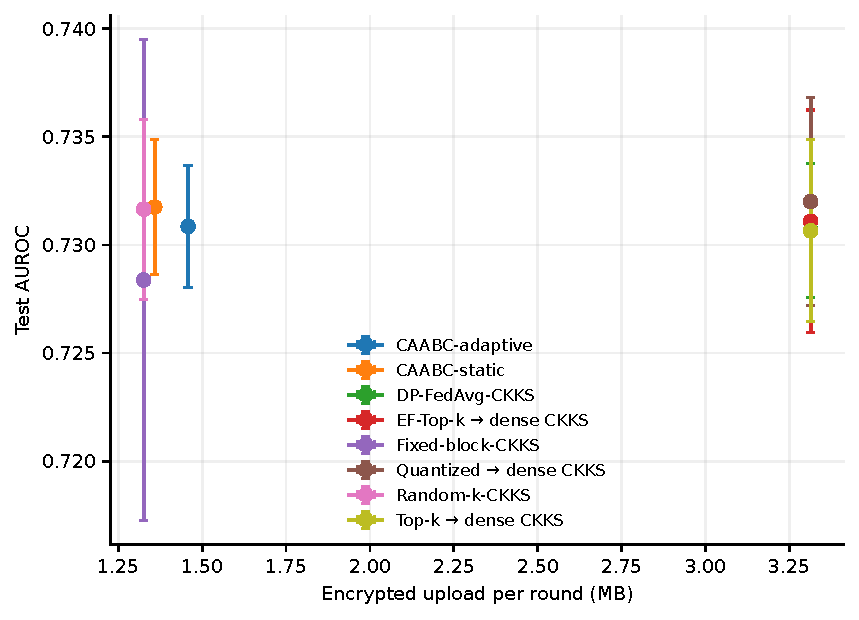
\includegraphics[width=0.88\textwidth]{utility_communication_pareto.pdf}
    \caption{Utility--communication relationship measured with serialized CKKS uploads. Error bars show 95\% confidence intervals across the applicable paired seeds.}
    \label{fig:utility-communication-pareto}
\end{figure}

\subsubsection{Poisoning behaviour}

The one-round poisoning matrix contained 870 registered conditions across attacks, malicious-client fractions, defences, and seeds. Figure~\ref{fig:poisoning-heatmap} summarizes the AUROC change at the most severe registered fraction of $40\%$ malicious clients. Ordinary weighted mean, which is compatible with sum-only CKKS aggregation, was highly vulnerable to model replacement and sign flipping. Model replacement reduced AUROC by $0.393$ on average, with a 95\% confidence interval from $-0.421$ to $-0.366$. It also increased backdoor ASR by $0.888$ on average.

\begin{figure}[htbp]
    \centering
    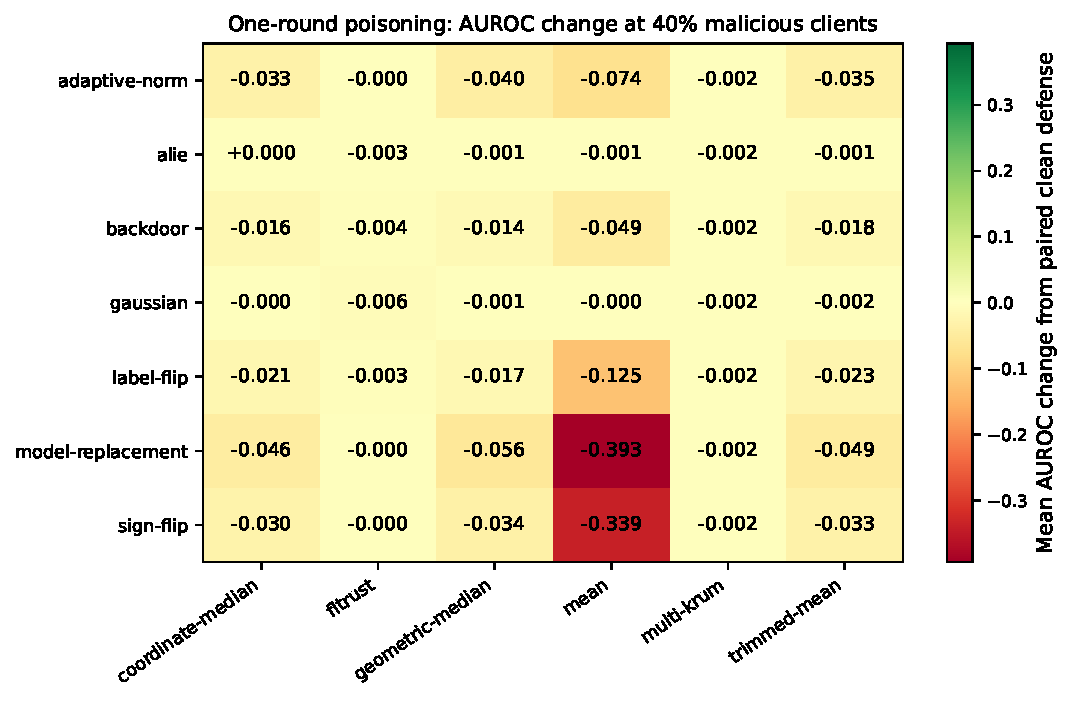
\includegraphics[width=\textwidth]{poisoning_heatmap.pdf}
    \caption{Mean AUROC change under one-round poisoning at 40\% malicious clients. Values are paired against a clean condition over five model seeds.}
    \label{fig:poisoning-heatmap}
\end{figure}

FLTrust and Multi-Krum controlled the registered one-round attacks more consistently than ordinary mean. However, both require information unavailable to the honest-but-curious coordinator in the main sum-only CKKS path: Multi-Krum requires pairwise geometry of individual plaintext updates, and FLTrust requires individual alignment with a labelled trusted-root update. They are therefore informative robustness comparators rather than drop-in replacements for the encrypted aggregator.

The five-round longitudinal experiment examined whether validation, rollback, and reputation could control attacks after aggregation. Table~\ref{tab:longitudinal-poisoning} reports the $40\%$ malicious-client cases. For the registered backdoor, the final ASR change was $0.0046$ with an interval crossing zero; every malicious client was quarantined, and $60\%$ of candidate rounds were rolled back. The same control reduced clean-task AUROC by $0.0293$, demonstrating that protection imposed an availability and utility cost.

\begin{table}[htbp]
    \centering
    \caption{Longitudinal validation and reputation results at 40\% malicious clients}
    \label{tab:longitudinal-poisoning}
    \resizebox{\textwidth}{!}{%
    \begin{tabular}{@{}lcccc@{}}
        \toprule
        Attack & Final AUROC change & Backdoor ASR change & Rollback rate & Quarantine recall \\
        \midrule
        Backdoor & $-0.0293$ [$-0.0413,-0.0173$] & $+0.0046$ [$-0.0501,+0.0592$] & 0.60 & 1.00 \\
        Model replacement & $-0.1066$ [$-0.3311,+0.1179$] & $+0.0610$ [$-0.0957,+0.2177$] & 0.60 & 1.00 \\
        Sign flip & $-0.1900$ [$-0.4681,+0.0882$] & $-0.0086$ [$-0.0795,+0.0624$] & 0.52 & 0.60 \\
        \bottomrule
    \end{tabular}}
    \vspace{1mm}

    \footnotesize Values are means and 95\% confidence intervals over five paired seeds. The control is aggregate-compatible but provides empirical release protection rather than a Byzantine guarantee.
\end{table}

\begin{figure}[htbp]
    \centering
    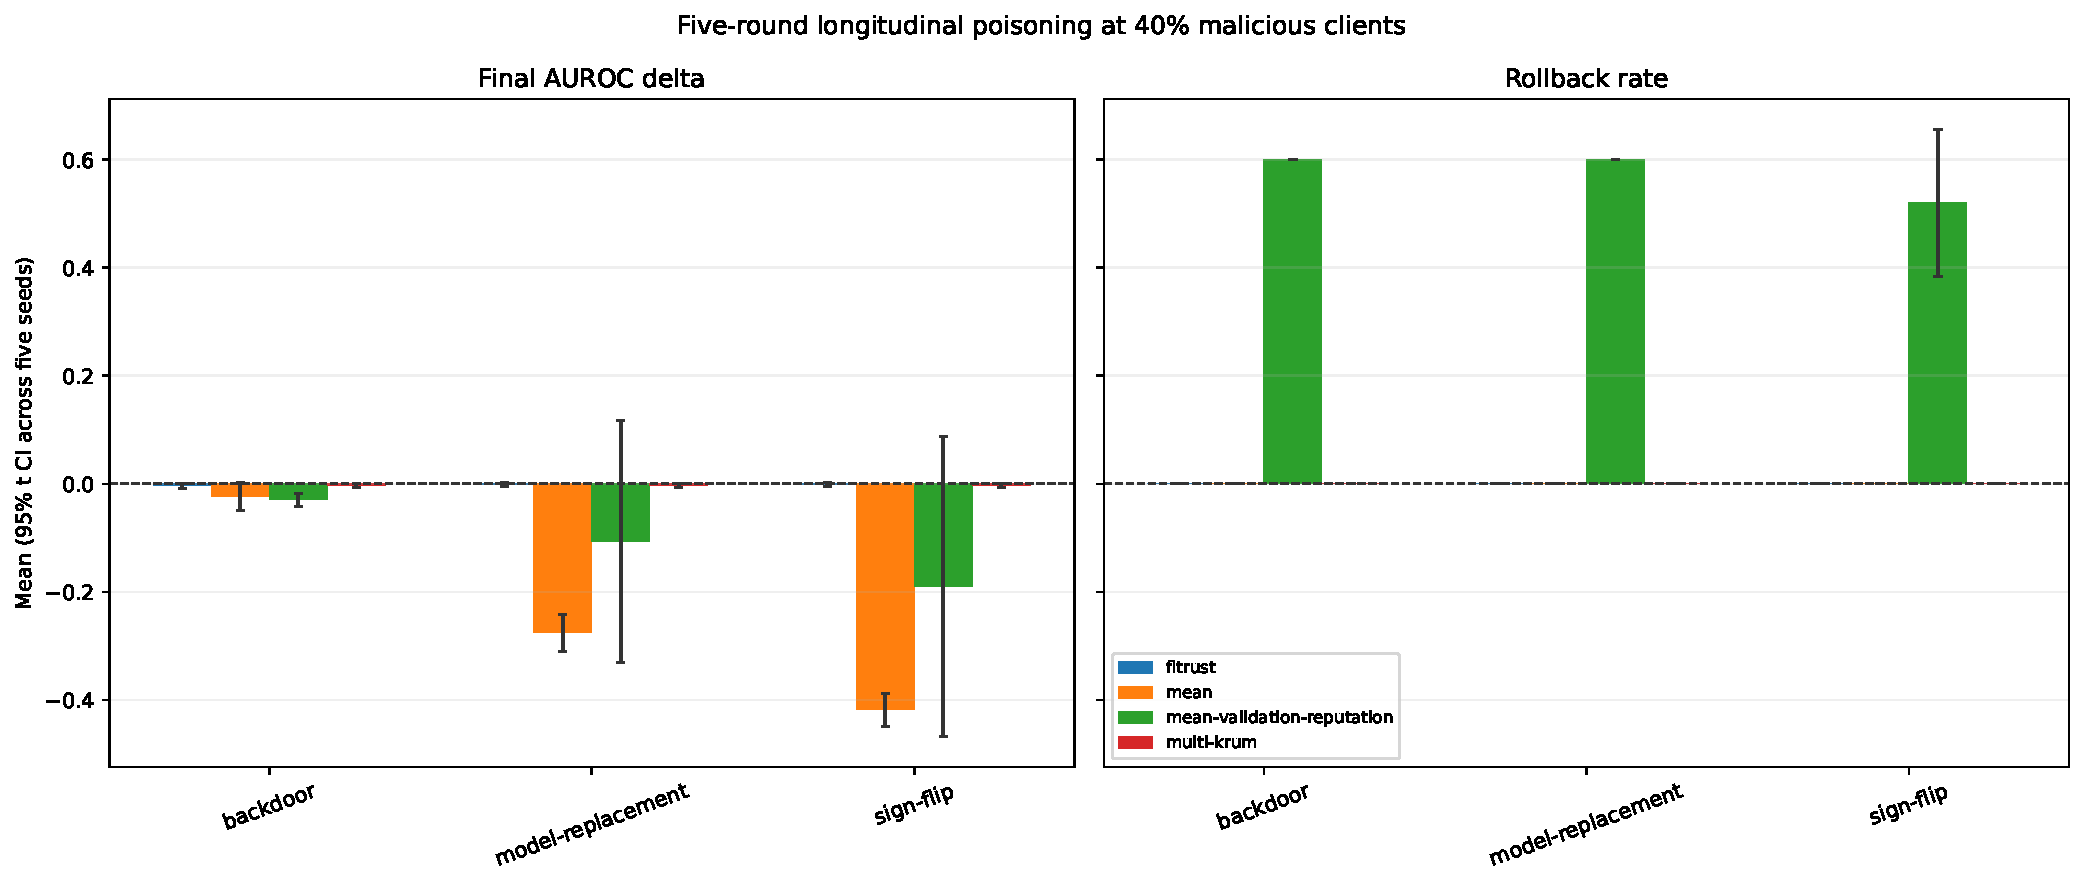
\includegraphics[width=\textwidth]{longitudinal_poisoning.pdf}
    \caption{Final utility change and rollback behaviour over five longitudinal poisoning rounds at 40\% malicious clients.}
    \label{fig:longitudinal-poisoning}
\end{figure}

\subsubsection{Membership inference and gradient reconstruction}

The powered loss-based membership experiment used 720 members and 720 non-members per model seed. FedAvg produced a mean attack AUROC of $0.5239$ [$0.5085$, $0.5393$]. Dense DP-FedAvg-CKKS produced $0.5050$ [$0.4922$, $0.5179$], while CAABC-FL produced $0.5035$ [$0.4929$, $0.5142$]. The CAABC-FL minus FedAvg paired difference was $-0.0204$ [$-0.0457$, $+0.0050$]. Because the interval crosses zero, the simple attack does not establish direct privacy superiority.

The stronger extension used architecture-matched reference models for online LiRA and low-cost RMIA diagnostics. Figure~\ref{fig:advanced-membership} shows both attack AUROC and true-positive rate at a 1\% false-positive rate. Under RMIA, FedAvg reached $0.5492$ [$0.5220$, $0.5763$], whereas dense DP-FedAvg-CKKS and CAABC-FL reached $0.5067$ [$0.4974$, $0.5161$] and $0.5063$ [$0.4969$, $0.5157$], respectively. Under online LiRA, the corresponding CAABC-FL value was $0.4963$ [$0.4886$, $0.5039$]. These findings show limited success for the registered attacks against the DP methods, while the formal privacy statement continues to come from the accountant rather than the empirical attack.

\begin{figure}[htbp]
    \centering
    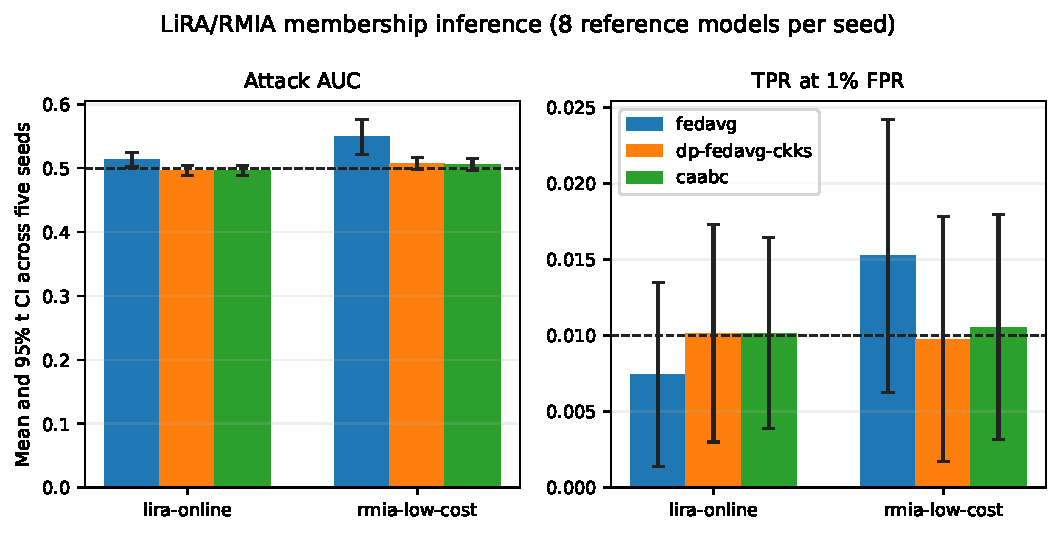
\includegraphics[width=\textwidth]{advanced_privacy.pdf}
    \caption{Advanced membership-inference evaluation using online LiRA and low-cost RMIA diagnostics with eight reference models per seed.}
    \label{fig:advanced-membership}
\end{figure}

Gradient reconstruction was run for 300 optimization steps on four records per seed over five model seeds. Table~\ref{tab:privacy-attack-results} and Figure~\ref{fig:gradient-reconstruction} show that DP-sanitized observations substantially increased reconstruction error. The plaintext-exact condition had a mean feature RMSE of $0.684$, while the DP-sanitized condition reached $2.547$. The worst-case DP plus CAABC exposure reached $2.763$, a paired increase of $2.079$ [$1.844$, $2.313$] relative to plaintext.

\begin{table}[htbp]
    \centering
    \caption{Confirmatory privacy-attack results}
    \label{tab:privacy-attack-results}
    \begin{tabularx}{\textwidth}{@{}lXcc@{}}
        \toprule
        Attack & Observation or method & Mean & 95\% confidence interval \\
        \midrule
        Membership & FedAvg attack AUROC & 0.5239 & [0.5085, 0.5393] \\
        Membership & DP-FedAvg-CKKS attack AUROC & 0.5050 & [0.4922, 0.5179] \\
        Membership & CAABC-FL attack AUROC & 0.5035 & [0.4929, 0.5142] \\
        Reconstruction & Plaintext-exact feature RMSE & 0.6844 & [0.4342, 0.9347] \\
        Reconstruction & DP-sanitized feature RMSE & 2.5467 & [2.3875, 2.7060] \\
        Reconstruction & DP+CAABC worst-case RMSE & 2.7632 & [2.5973, 2.9291] \\
        \bottomrule
    \end{tabularx}
\end{table}

\begin{figure}[htbp]
    \centering
    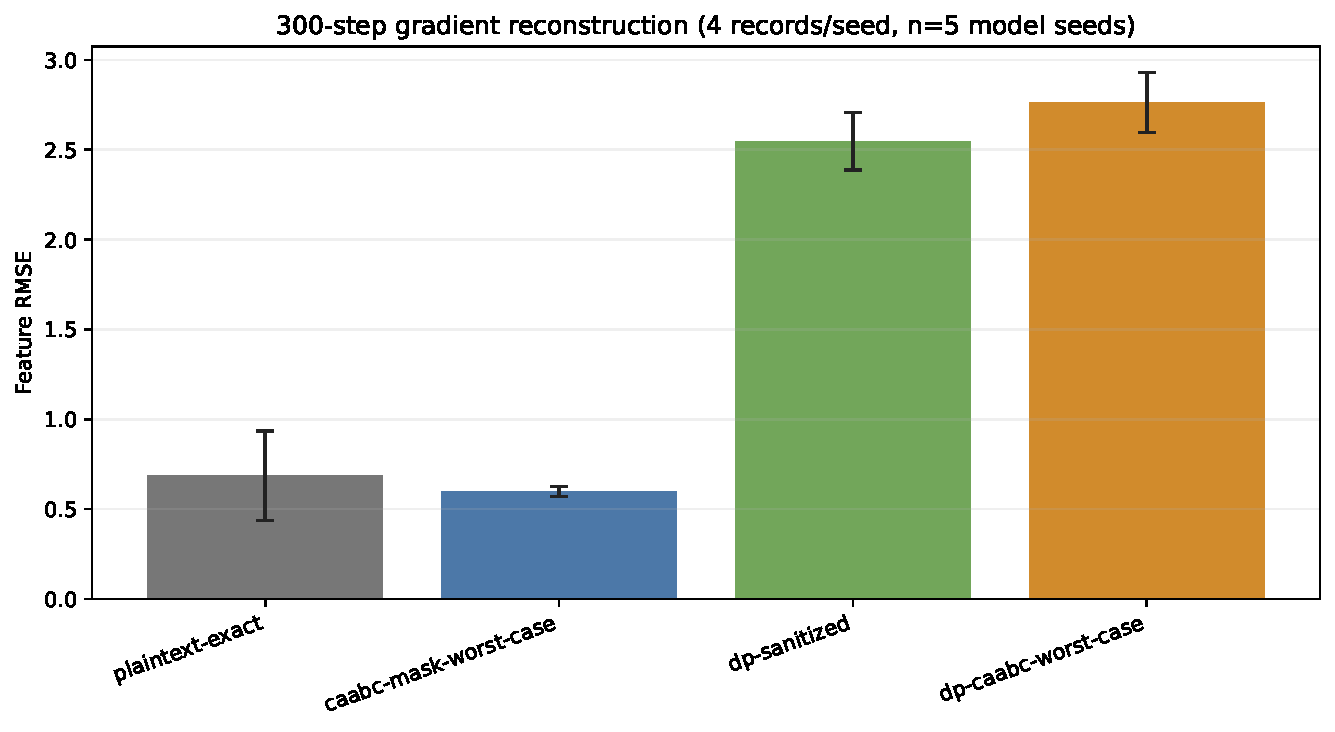
\includegraphics[width=0.92\textwidth]{gradient_reconstruction.pdf}
    \caption{Feature RMSE after 300-step gradient reconstruction. Higher error indicates a less accurate reconstruction under the registered optimizer.}
    \label{fig:gradient-reconstruction}
\end{figure}

The reconstruction experiment deliberately assumes that an attacker obtains a plaintext gradient after a hypothetical visibility failure. In the normal protocol, the coordinator receives a CKKS ciphertext and cannot directly run this attack. The result therefore measures an additional statistical protection layer rather than a break or validation of CKKS security.

\subsection{Statistical Analysis}
\label{subsec:results-statistics}

All principal comparisons were paired by seed so that each difference was calculated on the same patient split, initialization seed, and protocol configuration. Two-sided Student-$t$ 95\% confidence intervals were reported for effect estimation. Paired $t$-tests were accompanied by Wilcoxon signed-rank sensitivity tests where applicable, and Holm adjustment controlled multiplicity within the registered endpoint families. The primary conclusion was based on pre-specified decision gates rather than on isolated $p$-values.

The two co-primary gates compared CAABC-FL with dense DP-FedAvg-CKKS. AUROC non-inferiority used a margin of $-0.015$. The mean paired difference was $+0.00017$ with a 95\% interval of [$-0.00212$, $+0.00247$]. Because the lower confidence limit was above the margin, the AUROC gate passed. Actual encrypted-wire reduction used a minimum acceptable reduction of $40\%$. The observed mean was $55.998\%$ with an interval of [$55.994\%$, $56.002\%$], so the communication gate also passed. The co-primary decision was consequently positive.

\begin{table}[htbp]
    \centering
    \caption{Confirmatory CAABC-FL decision gates against dense DP-FedAvg-CKKS}
    \label{tab:confirmatory-gates}
    \begin{tabularx}{\textwidth}{@{}lccccX@{}}
        \toprule
        Endpoint & Margin or target & Mean effect & 95\% CI & Decision & Interpretation \\
        \midrule
        AUROC difference & $>-0.015$ & $+0.00017$ & [$-0.00212$, $+0.00247$] & Pass & Non-inferior within the registered margin \\
        Encrypted-wire reduction & $>40\%$ & $55.998\%$ & [$55.994\%$, $56.002\%$] & Pass & Target exceeded using serialized bytes \\
        AUPRC difference & Descriptive & $-0.00926$ & [$-0.01160$, $-0.00691$] & Adverse & Prevents a blanket superiority claim \\
        \bottomrule
    \end{tabularx}
\end{table}

The adverse AUPRC result is important. CAABC-FL lost $0.00926$ AUPRC relative to dense DP-FedAvg-CKKS, and the entire confidence interval was negative. It also increased the Brier score by $0.00211$ [$0.00177$, $0.00245$]. Thus, the statistically defensible conclusion is that CAABC-FL provides an AUROC-preserving communication trade-off, not that it is superior on every clinical metric.

The SOTA extension used five locked seeds and post-hoc locked non-inferiority margins of $0.015$ for AUROC and $0.020$ for AUPRC. CAABC-FL passed all eight one-sided method--metric non-inferiority tests after Holm correction. These tests show that the observed losses did not exceed the stated tolerances; they do not convert non-inferiority into superiority.

\section{Qualitative Results}
\label{sec:qualitative-results}

The qualitative evaluation examined whether the implemented components behaved according to their trust and policy contracts. No interviews, surveys, or clinical-user trials were conducted. Consequently, this section reports reproducible system cases and observed control behaviour rather than opinions attributed to users or clinicians.

\subsection{Visualization of Results}
\label{subsec:qualitative-visualization}

The main visual pattern across the scientific experiments is a three-way trade-off. Non-private optimizers occupy the highest discrimination region, dense DP and CKKS methods provide privacy and confidentiality at a utility and communication cost, and CAABC-FL moves the encrypted methods toward lower traffic while retaining similar AUROC. Security visualizations reveal a second pattern: controls that see individual plaintext updates are more effective against one-round poisoning, whereas aggregate-compatible validation and rollback act later by preventing release of a harmful candidate. Privacy plots show that the registered attacks become less effective after DP, but their near-chance outcomes are treated as empirical diagnostics rather than formal guarantees.

The service-scaling visualization in Figure~\ref{fig:service-scalability} reports the behaviour of the real mTLS/CKKS service with 18,049-coordinate updates. Sequential end-to-end latency increased from $1.337$ seconds for two clients to $7.080$ seconds for sixteen clients. Encrypted upload increased from $3.16$ MiB to $25.28$ MiB. A descriptive linear fit yielded approximately $413.5$ milliseconds per additional client with $R^2=0.9996$.

\begin{figure}[htbp]
    \centering
    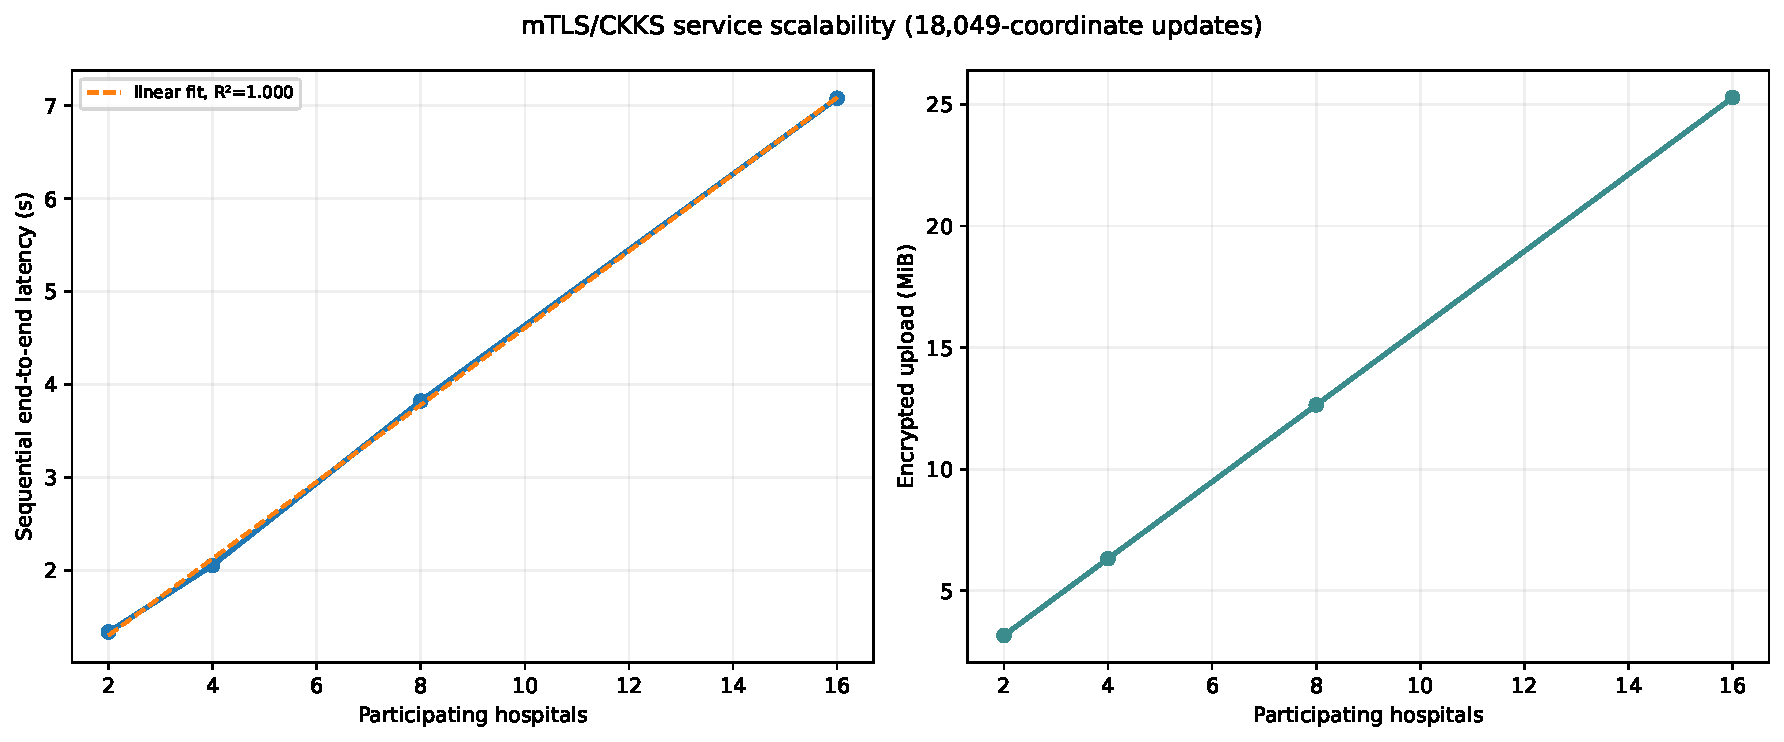
\includegraphics[width=\textwidth]{service_scalability.pdf}
    \caption{Single-host service-scaling diagnostic for two to sixteen clients using mTLS and real TenSEAL CKKS updates.}
    \label{fig:service-scalability}
\end{figure}

The near-linear curve is an observation from one sequential run per client count, not a throughput law. It does not include WAN delay, parallel submissions, peak resource utilization, real TDX/SNP hardware, or a physical multi-host cluster. The post-benchmark idle memory snapshot across the authority, coordinator, and three witnesses totalled approximately $291.4$ MiB, but this value is not a peak-memory measurement.

\subsection{User Evaluation and System Case Studies}
\label{subsec:case-studies}

Because the framework is a research system rather than a certified clinical application, involving clinicians or patients in a usability study would have implied a maturity that the implementation had not reached. Instead, case-based tests were used to examine security and governance behaviour. Table~\ref{tab:system-case-results} summarizes the principal observations.

\begin{table}[htbp]
    \centering
    \caption{Observed behaviour in governance, verification, and failure cases}
    \label{tab:system-case-results}
    \begin{tabularx}{\textwidth}{@{}lXX@{}}
        \toprule
        Case & Expected control & Observed result \\
        \midrule
        Authorized inference & Release only after consent, purpose, version, and guardian checks & Coarse risk output released after the required authorization \\
        Replay attempt & Reject a reused nonce & Request rejected as a replay \\
        Wrong purpose & Deny a purpose not covered by consent & Request rejected as purpose-not-consented \\
        Insufficient release quorum & Prevent unilateral release & Request rejected when the 2-of-3 authorization quorum was absent \\
        Consent revocation & Deny later release and remove retained ciphertext & Post-revocation request denied; retained ciphertext count became zero \\
        Forged aggregate & Recompute from original signed envelopes & Authority-side digest mismatch caused rejection \\
        Witness outage & Preserve release with the configured quorum & One of three witnesses could fail while two signed receipts completed the checkpoint \\
        Witness recovery & Restore chain continuity & Lagging witness reconciled after restart \\
        Missing multiparty share & Prevent correct 3-of-3 decryption & OpenFHE partial-decryption fusion failed without all shares \\
        \bottomrule
    \end{tabularx}
\end{table}

Independent aggregation verification was exercised with signed hospital envelopes. The authority reverified hospital signatures and participant digests, reconstructed the record weights, recomputed the ciphertext aggregate, and compared the resulting digest before decryption. A deliberately forged aggregate was rejected. This demonstrates independent recomputation, although it is not a zero-knowledge proof of correct computation.

The permissioned witness plane maintained three separately keyed services with a two-receipt release policy. Each witness verified the previous-hash and index continuity before signing a checkpoint. One witness outage was tolerated, and the lagging witness was reconciled after restart. These behaviours provide externally witnessed, tamper-evident evidence. They do not constitute Hyperledger Fabric, Raft, or Byzantine fault-tolerant consensus.

The isolated OpenFHE test completed native 3-of-3 multiparty CKKS with a maximum absolute aggregation error of $1.34\times10^{-13}$. Missing one share prevented correct decryption. This validates distributed key shares for that isolated experiment, but the result is neither an arbitrary $t$-of-$n$ construction nor a dropout-tolerant key service integrated with the main application.

\section{Comparative Analysis}
\label{sec:results-comparative-analysis}

\subsection{Benchmark Comparison}
\label{subsec:benchmark-comparison}

The benchmark comparison was divided into three groups. Conventional optimizers established the utility available without formal privacy. Dense DP-FedAvg-CKKS provided the closest privacy and encryption reference. Fed-EF-SGD, Fed-EF-AMS, and SoteriaFL-SGD represented recent communication-aware methods evaluated under the same healthcare protocol. Fed-EF was reimplemented from the published method because an official implementation was not linked from its publisher page. The SoteriaFL recurrence was checked against its official implementation, but the present comparison adapted it to record-level DP-SGD, study-specific weighting, the model-delta gradient surrogate, and dense CKKS transport. The reported values are therefore same-protocol healthcare results rather than replications of the original papers' dataset scores.

Table~\ref{tab:sota-utility-results} reports the five-seed comparison. All five methods produced AUROC values between $0.727$ and $0.732$. CAABC-FL achieved $0.730$ [$0.727$, $0.734$] and reduced encrypted upload by approximately $56\%$. Fed-EF-SGD achieved nearly identical AUROC but no meaningful encrypted-wire reduction after its client-specific sparse update was hidden through dense CKKS. SoteriaFL-SGD attained a higher F1 score in this comparison, while CAABC-FL retained the lower communication cost.

\begin{table}[htbp]
    \centering
    \caption{Same-protocol comparison with reproduced communication-aware methods}
    \label{tab:sota-utility-results}
    \resizebox{\textwidth}{!}{%
    \begin{tabular}{@{}lccccc@{}}
        \toprule
        Method & AUROC & AUPRC & F1 & Balanced accuracy & Encrypted-upload reduction \\
        \midrule
        DP-FedAvg-CKKS & 0.731 [0.726, 0.736] & 0.394 [0.386, 0.402] & 0.299 [0.234, 0.364] & 0.660 [0.647, 0.673] & 0.0\% \\
        CAABC-FL & 0.730 [0.727, 0.734] & 0.384 [0.376, 0.393] & 0.245 [0.174, 0.316] & 0.654 [0.640, 0.667] & 56.0\% \\
        Fed-EF-SGD & 0.731 [0.726, 0.736] & 0.395 [0.387, 0.403] & 0.272 [0.213, 0.331] & 0.657 [0.649, 0.665] & 0.0\% \\
        Fed-EF-AMS & 0.732 [0.728, 0.736] & 0.341 [0.327, 0.355] & 0.263 [0.241, 0.285] & 0.661 [0.660, 0.662] & 0.0\% \\
        SoteriaFL-SGD & 0.727 [0.716, 0.738] & 0.392 [0.383, 0.401] & 0.339 [0.318, 0.361] & 0.662 [0.656, 0.669] & 0.0\% \\
        \bottomrule
    \end{tabular}}
    \vspace{1mm}

    \footnotesize Values are means and 95\% confidence intervals over five locked paired seeds. Reductions use real serialized CKKS traffic; values displayed as 0.0\% were within measurement noise of the dense reference.
\end{table}

\begin{figure}[htbp]
    \centering
    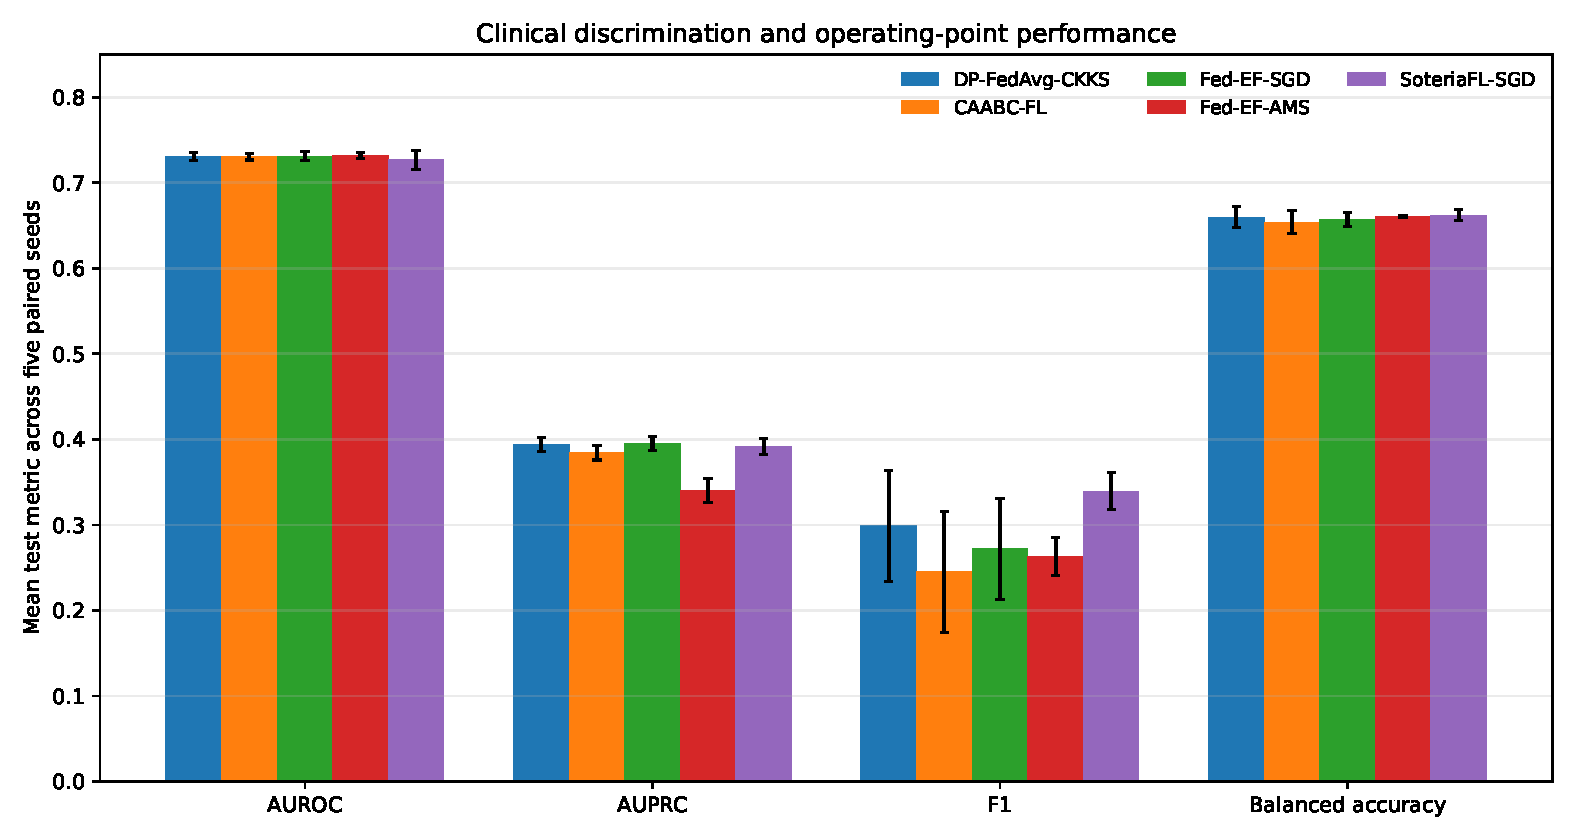
\includegraphics[width=\textwidth]{sota_clinical_metrics.pdf}
    \caption{Same-protocol predictive comparison over five paired seeds. Error bars show 95\% confidence intervals.}
    \label{fig:sota-clinical-metrics}
\end{figure}

Paired CAABC-FL differences further clarify the result. Against Fed-EF-SGD, the AUROC difference was $-0.0006$ [$-0.0048$, $+0.0037$], while the AUPRC difference was $-0.0106$ [$-0.0146$, $-0.0067$]. Against Fed-EF-AMS, CAABC-FL had an AUROC difference of $-0.0014$ [$-0.0036$, $+0.0008$] and an AUPRC advantage of $+0.0438$ [$+0.0314$, $+0.0562$]. Against SoteriaFL-SGD, its AUROC difference was $+0.0034$ [$-0.0062$, $+0.0131$] and its AUPRC difference was $-0.0076$ [$-0.0132$, $-0.0020$]. These mixed directions reinforce the interpretation of a design trade-off rather than universal superiority.

Figure~\ref{fig:sota-utility-wire} shows the property that most clearly separates CAABC-FL in the aligned comparison. Its utility interval overlaps the other private methods, but it is the only evaluated SOTA-style method that converts its compression into a substantial reduction in the actual encrypted upload under the imposed CKKS confidentiality rule.

\begin{figure}[htbp]
    \centering
    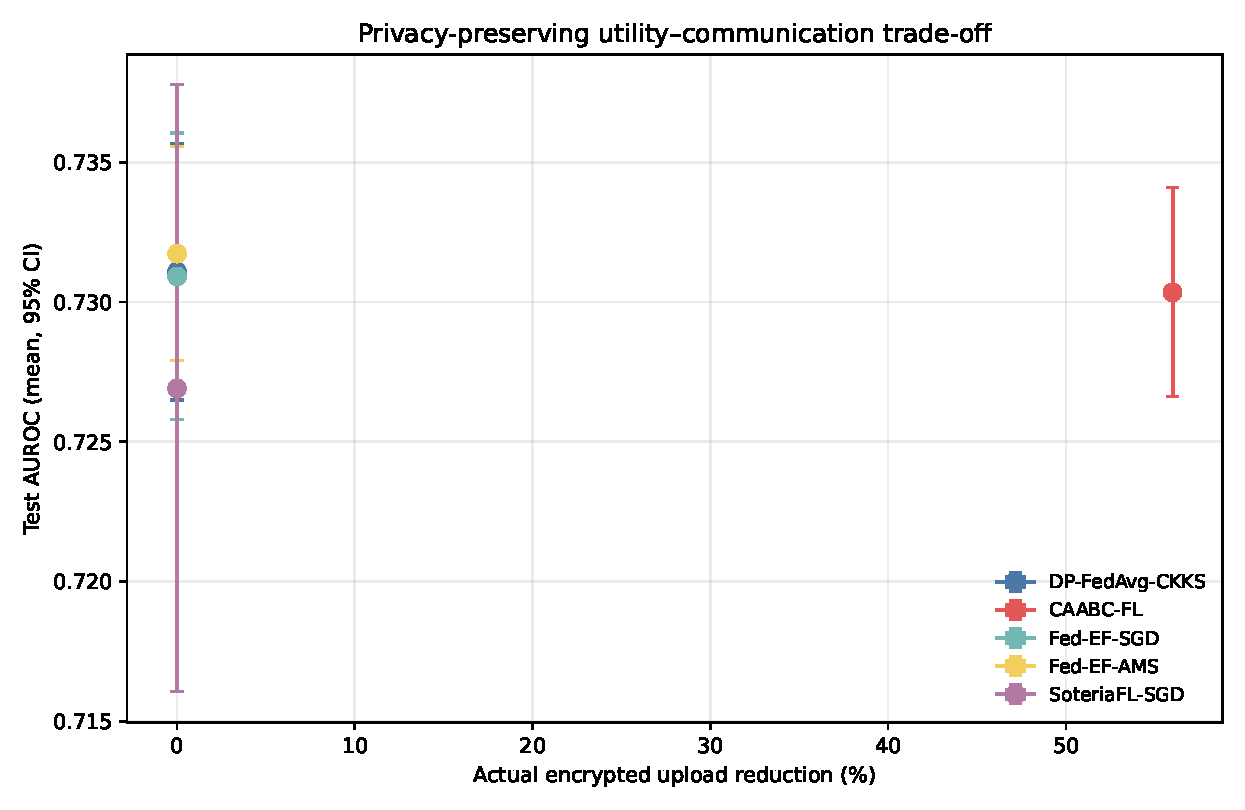
\includegraphics[width=0.88\textwidth]{sota_utility_wire_tradeoff.pdf}
    \caption{Same-protocol privacy-preserving utility and encrypted-communication trade-off.}
    \label{fig:sota-utility-wire}
\end{figure}

The broader comparison in Figure~\ref{fig:sota-security-systems} combines utility, advanced membership inference, one-round poisoning, and real CKKS microbenchmarks. The privacy results were similar among the DP methods. None of the compression schemes prevented the severe poisoning effect of ordinary weighted mean, confirming that compression is not a robustness mechanism. At sixteen clients, the CAABC-FL microbenchmark transmitted approximately $15.17$ MiB before amortizing support refresh, compared with roughly $25.28$ MiB for the dense encrypted methods. With a refresh interval of five rounds, its amortized upload was approximately $11.13$ MiB.

\begin{figure}[htbp]
    \centering
    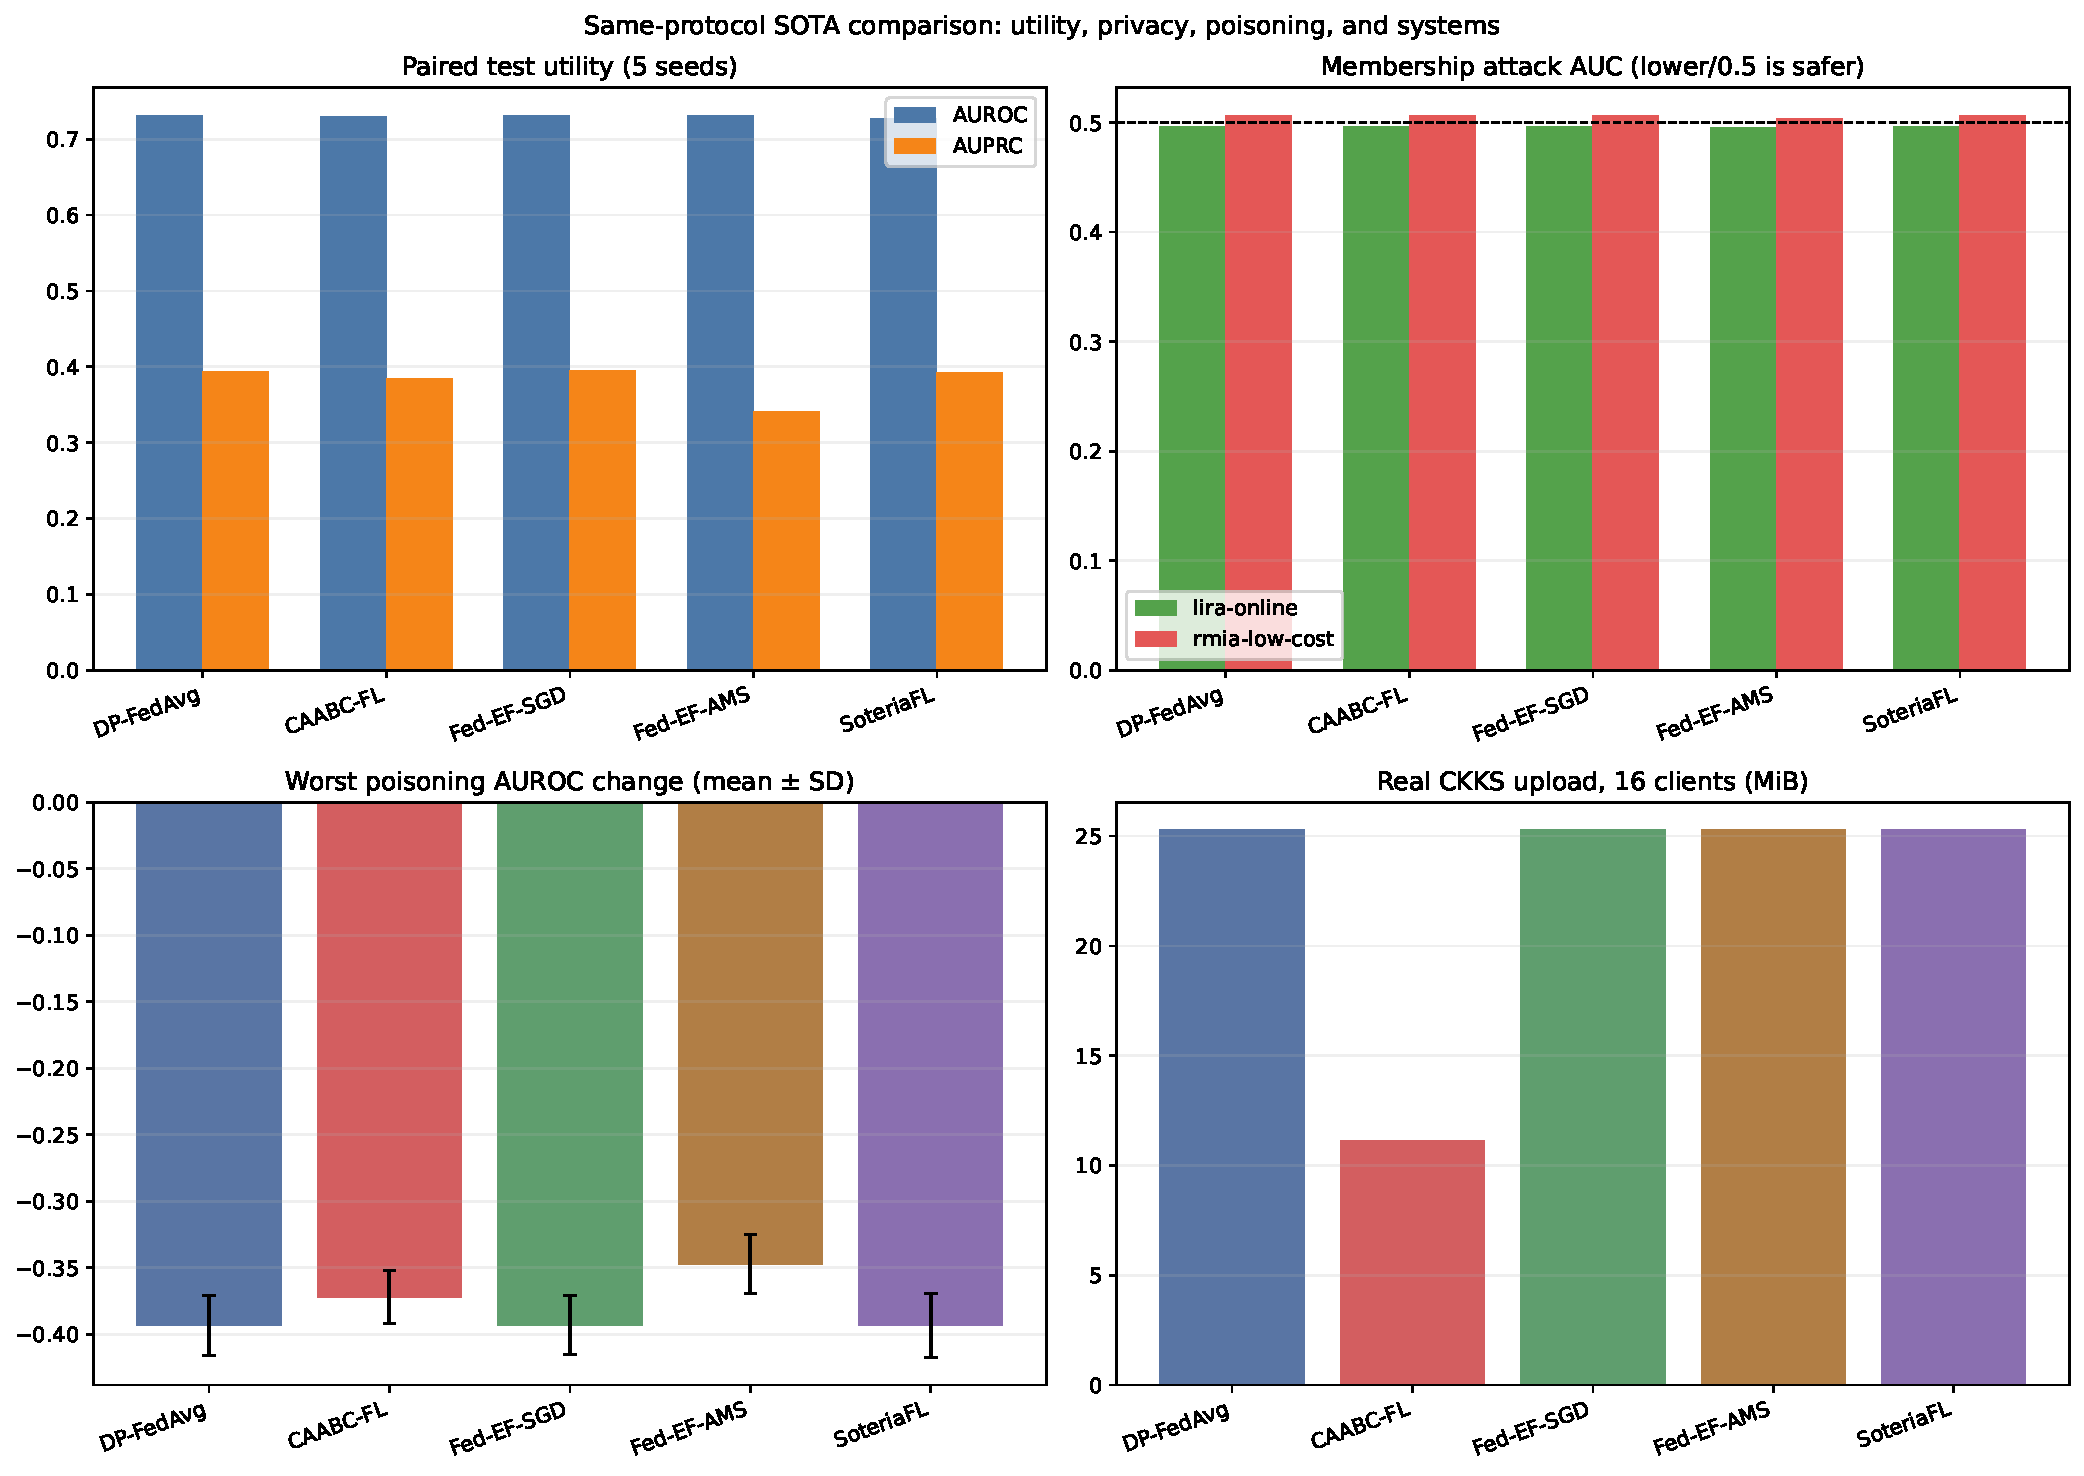
\includegraphics[width=\textwidth]{sota_security_systems.pdf}
    \caption{Same-protocol comparison across predictive utility, membership inference, poisoning sensitivity, and CKKS systems cost.}
    \label{fig:sota-security-systems}
\end{figure}

These systems values are real TenSEAL microbenchmarks, but they were measured in a single-process setting. The separate Docker service latency in Figure~\ref{fig:service-scalability} includes mTLS, persistence, verification, and audit operations and should not be numerically combined with the microbenchmark as though both measured the same execution path.

\subsection{Correlation with Literature Review}
\label{subsec:correlation-literature}

The non-private optimizer results agree with the literature reviewed in Chapter~\ref{chap:literature-review}: FedAvg provides a strong reference, while FedProx, SCAFFOLD, FedNova, FedAdam, and FedYogi alter the response to heterogeneity rather than guaranteeing a universal improvement \cite{mcmahan2017fedavg,li2020fedprox,karimireddy2020scaffold,wang2020fednova,reddi2021adaptive}. SCAFFOLD produced the highest non-private AUROC in the present matrix, $0.833$, but its advantage over the other non-private methods was small. This supports paired evaluation on the target hospital split instead of choosing an optimizer solely from results reported on unrelated datasets.

The reduction from non-private AUROC near $0.83$ to private AUROC near $0.73$ is consistent with the established utility cost of clipping and noise in DP-SGD \cite{abadi2016deep}. The comparison between plaintext DP-FedAvg and DP-FedAvg-CKKS indicates that this reduction was primarily associated with the DP training configuration rather than CKKS approximation. This finding is consistent with CKKS's purpose: it protects arithmetic inputs during aggregation but does not restore utility removed by privacy noise \cite{cheon2017homomorphic}.

The communication results extend the principle developed in Fed-EF and SoteriaFL that compression, privacy, and optimization should be analysed jointly \cite{li2023fedef,li2022soteriafl}. In this study, client-specific Top-$k$ and quantization reduced their logical representations but did not reduce the dense encrypted transport. CAABC-FL's contribution is therefore not simply another sparsifier. It aligns a common block support with CKKS packing so that the reported reduction is visible in serialized bytes. This observation also agrees with the broader design principle behind private block-sparse aggregation: the representation and privacy protocol must be co-designed \cite{asi2025preamble}.

The privacy results are consistent with modern membership-inference research in two ways. First, a simple average-case attack can understate leakage, motivating stronger likelihood-ratio and low-false-positive diagnostics \cite{carlini2022membership}. Second, empirical attack failure cannot substitute for a formal privacy statement. The present LiRA/RMIA and 300-step reconstruction experiments provide attack-specific evidence, whereas the $(\epsilon,\delta)$ claim is supplied by the record-level accountant. The higher reconstruction error after clipping and noise is also consistent with prior work showing that access to informative plaintext gradients is central to reconstruction success \cite{zhu2019dlg,geiping2020inverting}.

The poisoning experiments reproduce the central warning of the attack literature: linear averaging is highly vulnerable to model replacement and other manipulated updates \cite{bagdasaryan2020backdoor,fang2020local}. Krum, coordinate median, trimmed mean, geometric median, and FLTrust improved the registered one-round outcomes under their own assumptions \cite{blanchard2017krum,yin2018byzantine,pillutla2022robust,cao2021fltrust}. Their requirement for individual update geometry or a trusted labelled root explains why they cannot be presented as directly compatible with a sum-only CKKS coordinator. Integrated methods such as DDFed and DP-BREM+ address this privacy--robustness tension differently \cite{xu2024ddfed,gu2025dpbrem}; their published results remain contextual rather than direct numerical baselines because their datasets, cryptographic paths, and attacker models differ.

Finally, the trust-management observations support the literature's distinction between auditability and computation correctness. Permissioned ledgers can bind identities and preserve ordered records \cite{androulaki2018hyperledger}, but a recorded hash does not prove that an aggregate was computed correctly. The framework therefore combined witness receipts with authority-side recomputation. The isolated multiparty CKKS result is consistent with the distributed-custody direction of multiparty homomorphic encryption \cite{mouchet2021multiparty}, while its lack of dropout tolerance and network integration remains an explicit gap.

\subsection{Discussion of Improvements}
\label{subsec:discussion-improvements}

The clearest measured improvement is encrypted communication. CAABC-FL reduced serialized upload by approximately $56\%$ while passing the registered AUROC non-inferiority gate. This improvement came from three connected decisions: hospitals used a common block layout, selected blocks were aligned with CKKS packing boundaries, and omitted information was carried through error feedback. Without common support, client-specific indices would either leak structure or require dense re-encoding. Without ciphertext-aware accounting, a logical reduction could be mistaken for a network saving.

The ablation in Figure~\ref{fig:caabc-ablation} examines the block budget, support-refresh interval, and error-feedback mechanism. The registered $k=2$, refresh-five, error-feedback configuration achieved an AUROC of approximately $0.7303$ with a $56\%$ wire reduction. Reducing the budget to one block increased reduction to approximately $76\%$ while showing greater task-dependent utility variation. Increasing the budget to four or eight blocks progressively removed the communication benefit. Refreshing every round reduced the measured saving to approximately $40\%$, while refreshing every ten rounds increased it to approximately $58\%$. Removing error feedback produced a small mean AUROC decline of $0.0010$ relative to the registered configuration, with an interval crossing zero.

\begin{figure}[htbp]
    \centering
    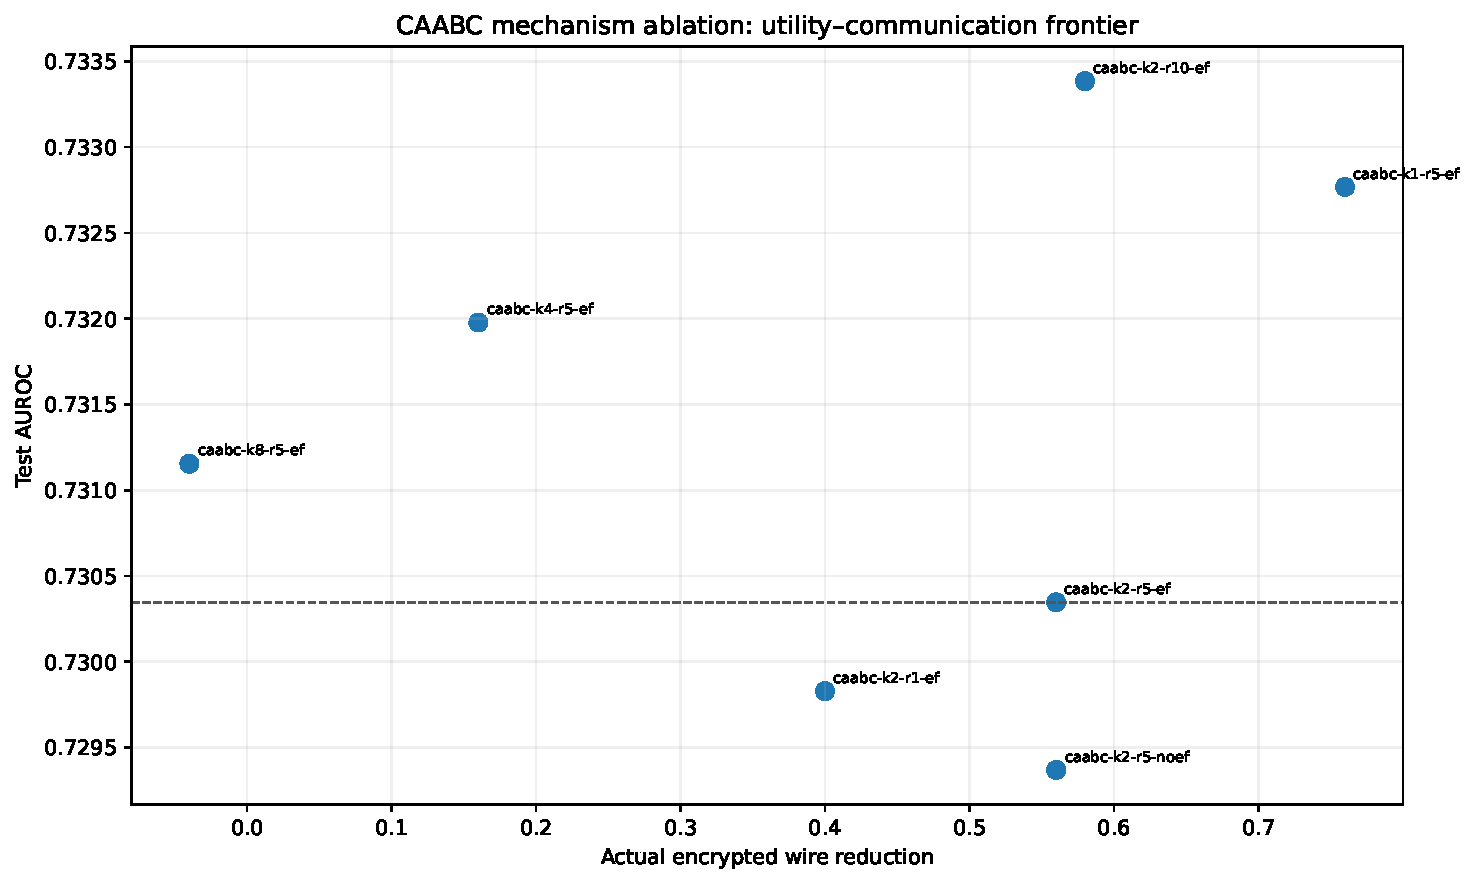
\includegraphics[width=0.92\textwidth]{caabc_ablation.pdf}
    \caption{CAABC-FL ablation showing the relationship between block budget, refresh policy, error feedback, AUROC, and actual encrypted-wire reduction.}
    \label{fig:caabc-ablation}
\end{figure}

The framework also improved accountability compared with a coordinator-only design. Hospital signatures, nonce and version binding, authority-side recomputation, atomic model registration, and two-of-three witness receipts created independent evidence around model release. These controls do not make the architecture decentralized, but they reduce the number of unchecked assumptions placed on the coordinator.

The poisoning results identify where improvement remains necessary. Validation and reputation protected the released state against the registered longitudinal backdoor, but they imposed rollback and clean-utility costs and did not provide a universal guarantee. A five-seed verified encrypted FLTrust experiment showed that certified norm and cosine sufficient statistics could reproduce the corresponding plaintext scalar aggregation with a maximum absolute error near $4.05\times10^{-8}$ and zero certified malicious weight in the tested failure case. However, the custodians in that experiment could observe the released norm and cosine statistics, and networked threshold computation of those statistics was not implemented. It is therefore evidence for a possible aggregate-compatible direction, not a completed replacement for the current validation gate.

\section{Discussion of Findings}
\label{sec:discussion-findings}

The first research objective was to design and implement a hybrid framework combining local data retention, record-level DP, encrypted aggregation, communication efficiency, poisoning controls, and accountable governance. The implementation met this objective at research-system level. Patient data remained local; the confirmatory private methods used a recorded $(\epsilon,\delta)=(1.935,10^{-5})$ configuration; model updates were protected with real TenSEAL CKKS; authenticated services used signatures and mTLS; and aggregation, model registration, and witness checkpoints were exercised. The evidence does not extend to regulatory approval, clinical deployment, or an attested physical multi-host environment.

The second objective was to develop and evaluate CAABC-FL as a privacy-safe, ciphertext-aware communication mechanism. The co-primary result supports this objective. Compared with dense DP-FedAvg-CKKS, CAABC-FL reduced encrypted upload by approximately $56\%$ and passed the AUROC non-inferiority margin. The result is stronger than a logical sparsity claim because it was measured from serialized ciphertexts. At the same time, AUPRC, F1, precision, specificity, and Brier score revealed adverse changes. The appropriate conclusion is therefore that CAABC-FL offers a useful operating point on the privacy--utility--communication frontier, not that it dominates every baseline.

The third objective was to evaluate the framework against privacy and integrity threats using reproducible comparisons. This objective was addressed through five-seed poisoning experiments, five-round longitudinal attacks, powered membership inference, advanced LiRA/RMIA diagnostics, 300-step gradient reconstruction, SOTA-aligned comparisons, and system failure cases. The results expose both strengths and weaknesses. DP methods resisted the registered membership and reconstruction attacks more effectively than the non-private or plaintext-exposure conditions. Validation, rollback, and reputation limited the registered longitudinal backdoor. However, ordinary encrypted mean remained vulnerable to one-round model replacement, and the post-aggregation gate introduced measurable utility and availability costs.

Three broader insights emerge. First, privacy, communication, and robustness cannot be evaluated independently. Encryption can prevent the coordinator from applying an otherwise effective plaintext robust aggregator; compression may provide no network benefit after encryption; and a strict poisoning gate may protect integrity by reducing availability. Second, multiple metrics are necessary. AUROC alone would hide the adverse AUPRC and operating-point changes, while attack AUC alone would hide the assumptions governing attacker visibility. Third, governance evidence must be separated from decentralization. Signed witnesses and independent recomputation increase accountability, but the main service still uses a centralized research key authority.

\begin{table}[htbp]
    \centering
    \caption{Research-objective outcomes and evidence boundaries}
    \label{tab:objective-outcomes}
    \begin{tabularx}{\textwidth}{@{}p{0.17\textwidth}p{0.42\textwidth}X@{}}
        \toprule
        Objective & Main evidence & Boundary \\
        \midrule
        Hybrid secure framework & Real DP training, CKKS aggregation, authenticated services, independent recomputation, model registry, and witness receipts & Research system; not a certified clinical or physical multi-host production deployment \\
        CAABC-FL communication method & 55.998\% encrypted-wire reduction and passed AUROC non-inferiority gate & AUPRC and several operating-point metrics declined; no universal superiority \\
        Privacy and attack evaluation & Five paired seeds, powered membership inference, 300-step reconstruction, one-round and longitudinal poisoning, and failure cases & Valid for the registered cohort, attacks, visibility, and software testbed only \\
        \bottomrule
    \end{tabularx}
\end{table}

Several limitations constrain external validity. The clinical evidence comes from one challenge cohort with two natural hospital systems and one matched-landmark sepsis task. No independent external clinical dataset or prospective evaluation was performed. The service-scaling test used one physical Docker host, so it does not measure WAN communication, concurrent hospital behaviour, or failure across independent administrative networks. The custom secure random-number implementation was recorded and exercised but has not received an independent cryptographic audit. The main TenSEAL service uses one centrally held research secret key. The separate OpenFHE experiment demonstrates 3-of-3 multiparty CKKS only; it is not integrated, arbitrary threshold, or dropout tolerant. The Kubernetes confidential-computing profile passed schema validation but was not executed on real Intel TDX or AMD SEV-SNP hardware.

Within these boundaries, the study provides a defensible answer to the research problem. Secure collaboration is possible without moving raw hospital records, but its quality cannot be summarized by accuracy alone. The strongest contribution is the experimentally demonstrated alignment of adaptive compression with encrypted transport: CAABC-FL reduces real CKKS traffic while retaining dense-reference AUROC within a registered margin. The security results add a necessary qualification: encrypted efficiency does not remove poisoning risk, and governance controls must be evaluated together with their utility and availability costs. Future work should therefore prioritize external clinical validation, integrated networked threshold custodians, secure robust statistics under encryption, physical multi-host testing, and hardware-attested key release rather than broadening the present claims beyond the produced evidence.
